% !TeX spellcheck = <none>
\documentclass[11pt,a4paper]{article}
\usepackage{geometry}
\geometry{a4paper,left=25mm,right=25mm, top=24mm, bottom=24mm}

\usepackage{amsmath,amssymb,amstext,amsthm}
\usepackage{optidef}
%\usepackage{ucs}
\usepackage[utf8x]{inputenc}
%\usepackage[T1]{fontenc}
\usepackage[ngerman]{babel}
%\usepackage[ngerman]{varioref}
\usepackage{xcolor}
\usepackage{babelbib}
\usepackage[hidelinks]{hyperref}
\usepackage{tikz}
\usepackage{tikz-cd}
\usepackage{caption}
\usepackage[linesnumbered]{algorithm2e}
\usepackage{pgfplots}




\DeclareMathOperator*{\Max}{max}
\newcommand{\N}{\mathbb{N}}
\newcommand{\Z}{\mathbb{Z}}
\newcommand{\Q}{\mathbb{Q}}
\newcommand{\TODO}{\textcolor{red}{TODO}}

\newtheoremstyle{my_th_style1}%
{6pt}%		// space above
{0pt}%		// space below
{}%		// body font
{}%		// indent amount
{\bfseries}%	// theorem head font
{:             }%		// punctuation after theorem head
{.5em}%	// space after theorem head
{}%		// theorem head spec

\theoremstyle{my_th_style1}
\newtheorem{satz}{Satz}

\makeatletter 
\renewenvironment{proof}[1][\proofname]{\par 
	\pushQED{\qed}% 
	\normalfont \topsep6\p@\@plus6\p@\relax 
	\trivlist 
	\item[\hskip\labelsep 
	%         \itshape 
	\bfseries 
	#1\@addpunct{:}]\ignorespaces 
}{% 
\popQED\endtrivlist\@endpefalse 
} 
\makeatother 

%opening
\title{Projekt 2: Fiber-To-The-x}
\author{Moritz Hefner und Lucia Ortjohann}

\begin{document}
\maketitle
\thispagestyle{empty}
\newpage
\tableofcontents
\thispagestyle{empty}
\newpage
\setcounter{page}{1}

%\section{PROBLEME}
% \begin{itemize}
%	\item DISKUNKTE VEREINGIGUNG VON WEGEN GENAUER ERKLÄREN
% 	\item ALLLES SSOOOOO HÄÄSSLICH
% 	\item P2PG was tun wir genau?
% 	\item Problemstellung auch die PRObleme genau beschreiben oder nur die %Daten und wann beschreibe ich welches Problem nochmal
 %	\item Name für Facility
 %	\item constraint in das modell/die modelle einfügen für assEdges = 0 falls endknoten nicht mit customer uebereinstimmt
% \end{itemize}


\section{Problemstellung}

Dieses Projekt behandelt die Problemstellung in einem Netzwerk von Kunden und Verbindungswegen diese Kunden mit einer Internetverbindung aus einer Leitstelle zu versorgen.
Dabei k\"onnen die Kunden entweder via Glasfaser- oder \"uber Kupferkabel mit jeweils verschiedenen Kosten und verschiedenen Bandbreiten angeschlossen werden.
Jeder Kunde besitzt eine individuelle Nachfrage an Bandbreite, die gedeckt werden muss.
Gesucht ist ein kosteng\"unstigster Standort f\"ur eine Leitstelle mit einer Verbindung von dieser zu jedem Kunden.
Dabei unterscheiden wir zwischen zwei verschiedenen Problemstellungen.
Beim Point-to-point (P2P) Problem soll jeder Kunde eine eigene Glasfaserleitung bis zur letzten Anschlusskante (letzte Meile) bekommen.
Dahingegen dürfen beim Point-to-multipoint (P2MP) Problem sogenannte Splitter installiert werden, die mehrere Glasfaserkabel zusammenfassen k\"onnen.
 
Wir formulieren und lösen diese Probleme auf einem Graphen \(G=(V,A)\).
Dabei besteht die Knotenmenge aus vier disjunkten Mengen $L,K,F,S \subseteq V$, wobei $L$ die Menge der m\"oglichen Leitstellen ist. Weiterhin ist $K$ die Menge der zu versorgenden Kunden und $F$ ist eine Menge von so genannten Facility Knoten.
Von einer Facility aus können Kunden mit Glasfaser oder Kupfer angeschlossen werden.
Die Menge $F_1 \subseteq F$ ist die Menge der Facility Knoten von Typ 1.
Von diesen aus können Kunden ausschließlich über Glasfaserverbindungen angeschlossen werden.
Die Facility Knoten, von denen Kunden mit Kupfer angeschlossen werden können, bilden die Menge $F_2$. Dabei sind die Mengen $F_1$ und $F_2$ disjunkt.
Ferner bildet $S$ die Menge der Knoten, die für die Verbindung der Facility Knoten zu einer Leitstelle genutzt werden k\"onnen (Steinerknoten). 

Die Menge der Kanten $A$ besteht aus den inneren Kanten $I$, die ausschließlich Knoten aus \(L, S\) und \(F\) miteinander verbinden, und den Anschlusskanten, wobei unterschieden wird, ob diese Verbindung mit Glasfaser \(A_1\) oder Kupfer $A_2$ möglich ist.
Dabei sind die Kantenmengen $A_1$ und $A_2$ disjunkt.
Eine Anschlusskante geht immer von einem Knoten der Menge $F$ zu einem Kunden $k \in K$. 
Im Folgenden betrachten wir $G$ als gerichteten Graphen.
Dazu fassen wir die Anschlusskanten als Kanten von der Facility zum Kunden auf.
Für jede innere Kante $ij \in I$, außer für die Kanten mit $i \in L$, fügen wir zusätzlich noch die Kante $ji$ zu $I$ mit identischen Kosten hinzu.
Dieser Graph bildet das Grundgerüst für unsere Probleme.

Das Ziel ist ein kosteng\"unstigstes Netzwerk zu finden, sodass alle Forderungen erf\"ullt sind.
Dazu ist die Kostenfunktion 
\begin{align}
\label{Kostenfunktion}
c: V \cup A \rightarrow \Q_{\geq 0}
\end{align}
 gegeben.
Für die Verlegung von Glasfaser auf den inneren Kanten $I$ und f\"ur die Verlegung von Kupfer auf den Anschlusskanten \(A_2\) von Typ 2 fallen Kosten in Höhe von $c(e)$ mit $e \in I \cup A_2$ an.
Die  Anschlusskanten von Typ 1 haben die Länge 0 und verursachen somit keine Kosten.
Der Aufbau einer Leitstelle $ l\in L$ kostet $c(l)$. 
In den Facility Knoten kann man entweder einen DSL-Zugangsmultiplexer (DSLAM) installieren, falls ein Facility Knoten von Typ 2 vorliegt, oder an einen Facility Knoten von Typ 1 einen Kunden an Glasfaser anschließen.
Dabei ist zu beachten, dass ein Kunde lediglich dann \"uber ein Kupferkabel von einem Facility Knoten angeschlossen werden kann, wenn in diesem ein DSLAM installiert ist.
Dafür entstehen Kosten in Höhe von $c(f)$ für alle $f \in F_2$.
Zusätzlich hat jeder Kunde \(k \in K\) noch eine Nachfrage an Bandbreite von $d(k)$ und für den Anschluss eines Kunden kann mit Profit von $p_1(k)$ für einen Anschluss mit Glasfaser und $p_2(k)$ für einen Anschluss mit Kupfer gerechnet werden.
Außerdem entstehen bei P2MP noch Kosten für die Installation eines Splitters in H\"ohe von $c_s$.
Ein Splitter darf in einen Steinerknoten oder einen Facility Knoten installiert werden, sofern dort kein DSLAM installiert wird, und kann ein eingehendes Glasfaserkabel in bis zu 4 (16) ausgehende Glasfaserkabel aufteilen.

Die Ergebnisse der einzelnen Probleme auf drei vorgegebenen Instanzen werden jeweils am Ende der Abschnitte beschrieben.
Um die Laufzeiten der Algorithmen besser vergleichen zu können, geben wir nun die technischen Daten der genutzten Computer an:
\begin{table}[h]
	\centering
	\begin{tabular}{|c|p{5.5cm}|c|c|}
		\hline
		Computer & \centering{Prozessor} & RAM & Betriebssystem \\	
		\hline
		PC 1 &Intel(R) Core(TM) i7-4500 CPU @ 1.80GHz x 4 & 8,00 GB & Ubuntu 18.04.1 LTS\\
		PC 2 & Intel(R) Core(TM) i5-2430 CPU @ 2.40GHz & 8,00 GB & Windows 10 Home Premium\\
		PC 3 & 4 x Intel(R) Xeon(R) CPU @ 2.93GHz  & 12,30 GB & \\%Linux linux 3.13.0-162-generic #212-Ubuntu SMP Mon Oct 29 12:08:50 UTC 2018 x86_64 x_86_64 x86_64 GNU/Linux\\
		\hline 
	\end{tabular}
	\caption{Technische Daten} 
\end{table}
\newpage

\section{Vorüberlegung}
\label{preprocess}

Um jeden Kunden seinem Bedarf entsprechend zu versorgen, muss die Nachfrage jedes Kunden gedeckt sein.
Diese Bedingungen k\"onnen wir mit einfachen Vor\"uberlegungen decken.

Da die Kapazität der Glasfaserleitungen in unserem Modell unendlich ist, wird die Nachfrage eines Kunden auf jeden Fall gedeckt, wenn dieser mit Glasfaser angebunden ist.
Außerdem kann auf den inneren Kanten nur Glasfaser verlegt werden.
Das heißt, die einzigen Kanten, die dafür sorgen könnten, dass die Nachfrage eines Kunden nicht gedeckt ist, sind die Anschlusskanten von Typ 2.
Diese gehen von einer Facility zu einem Kunden und falls die Kapazit\"at dieser Kante nicht mindestens der Nachfrage des Kunden entspricht, können wir diese in unserem Netzwerk nicht benutzen. 
Deswegen löschen wir, bevor wir die verschiedenen Probleme lösen, s\"amtliche Anschlusskanten von Typ 2, die die Nachfrage des jeweiligen Kunden nicht decken k\"onnen, aus dem oben genannten Graphen.
Daher erf\"ullt jedes Netzwerk in dem neuen Graphen somit die Nachfrage aller Kunden.
Damit betrachten wir die Nachfrage der Kunden nicht mehr, bis wir zu einer Erweiterung der Problemstellungen auf eine m\"ogliche Erh\"ohung der Nachfrage der Kunden kommen.
Diesen neuen Graphen bezeichnen wir im Folgenden wieder mit $G=(V,A)$ und lösen die folgenden Probleme auf diesem Graphen.
Da die gelöschten Kanten in keiner der Lösungen benutzt werden könnten, verändert dies die Lösungen nicht.

\section{Point-to-point}

Wir behandeln im Folgenden die P2P Problemstellung.
Zuerst betrachten wir den Fall, dass s\"amtliche Kunden \"uber Glasfaserkanten angeschlossen werden m\"ussen.
Danach analysieren wir die Variante, dass sowohl Kupfer- als auch Glasfaserverbindungen erlaubt sind und zum Schluss dieses Kapitels ber\"ucksichtigen wir die M\"oglichkeit, dass die Kunden \"uber verschiedene Anschlusskanten auch unterschiedliche monatliche Profite f\"ur das Telekommunikationsunternehmen generieren oder die Nachfrage nach Bandbreite sich erh\"oht.

\subsection{Point-to-point mit Glasfaser}

Beim P2P mit Glasfaser Problem (P2PG) muss jeder Kunde mit einer eigenen Glasfaserleitung angeschlossen werden.
Unser Problem besteht also darin, eine Leitstelle aus $L$ auszusuchen und dann ein Glasfaserkabel von dieser Leitstelle zu einem Facility Knoten von Typ 1 zu verlegen, um dann mit der Anschlusskante von der Facility zum Kunden den Kunden anzubinden.
Dabei sollen die anfallenden Kosten minimiert werden.
Es gibt f\"ur jeden Kunden genau eine Anschlusskante und eine Facility von der dieser Kunde mit Glasfaser angebunden werden kann und die Länge dieser Kante ist 0.
Damit kann man das Problem einen Kunden anzuschließen, auch als kürzestes Weg Problem von einer Leitstelle zu der Facility des Kunden betrachten.
Wir lösen also für jede Leitstelle in $L$ einmal das kürzeste Wege Problem zu jeder Facility von Typ 1.

Dabei gehen wir wie folgt vor:
Für jede Leitstelle $ l \in L$ berechnen wir auf dem Hilfsgraphen $H=(\{l\} \cup S \cup F , I,c\mid_I)$ einen kostenminimalen Weg von der Leitstelle $l$ zu jeder Facility $f \in F_1$. Dazu führen wir den Algorithmus von Dijkstra zur Berechnung k\"urzester Wege einmal mit Startknoten $l$ durch.
Der errechnete Weg zur Facility \( f \in F_1\) sei nun $W_{l,f}$ und die Kosten dieses Weges seien $c_{\text{dij}}(lf)$. 
Jeder Kunde besitzt nur eine eingehende Anschlusskante von Typ 1, diese hat Verlegungskosten 0.
Andersherum besitzt jede Facility aus $F_1$ genau einen Kunden, den diese anschließen muss. 
Daher sind die Kosten der optimalen Lösung für die ausgewählte Leitstelle $l$ nun $C_l:=c(l) + \displaystyle\sum_{f \in F_1} c_{\text{dij}}(lf) + c(f)$. 
Nun suchen wir die Leitstelle $i \in L$ mit den geringsten Kosten ($i:=\arg \displaystyle\min_{l \in L} C_l$).
Das zugehörige Netzwerk setzt sich aus den errechneten kürzesten Wegen $W_{i,f}$ für alle $f \in F_1$ und allen Anschlusskanten von Typ 2 zusammen, also ist das Netzwerk die Menge $(\bigsqcup_{f \in F_1 }W_{i,f}) \cup A_2 $.
Die disjunkte Vereinigung bedeutet, dass falls zwei Wege über dieselbe Kante laufen, wir in unserem Netzwerk auch zwei Glasfaserkabel über diese Kante verlegen.

In diesem Algorithmus wenden wir also $|L|$ Mal den Dijkstra-Algorithmus an.
Dieser hat eine polynomielle Laufzeit von \(\mathcal{O} ( {|\{l\} \cup S \cup F |}^2 )\).

\textbf{Ergebnisse:} Die errechneten Kosten und die Laufzeiten sind in der folgenden Tabelle 2 dargestellt.
Die Ergebnisse  der verschiedenen Probelme vergleichen wir in unserer Zusammenfassung.
\begin{table}[h]
	\centering
	\begin{tabular}{c|c|c|c}
		 Instanz & Naunyn & Berlin & Vehlefanz \\	
		\hline
		Kosten & 480.722 & 1.388.562 & 7.791.258 \\
		\( |\{l\} \cup S \cup F | \) & 9 & 381 & 891 \\
		Laufzeit auf PC2 & 0,001s & 0,26s & 2,35s\\
	\end{tabular}
	\label{P2PG}
	\caption{Ergebnisse des P2PG} 
\end{table}
Die Abbildungen \eqref{p2pg_n_pic}, \eqref{p2pg_b_pic} und \eqref{p2pg_v_pic} im Anhang sind graphische Darstellungen der L\"osungen zu allen drei Instanzen.



\subsection{Point-to-point mit Glasfaser und Kupfer}
Das Point-to-point mit Glasfaser und Kupfer Problem (P2PGK) ist eine Erweiterung des P2PG Problems.
Hierbei d\"urfen Kunden nun auch \"uber Kupferkabel angeschlossen werden.
Dabei k\"onnen diese Kupferkabel lediglich als letzte Verbindungskanten von einer Facility von Typ 2 zu einem Kunden verlegt werden.
Ferner muss, falls ein Kunde von einer Facility \(f \in F_2\) aus mit Kupfer angeschlossen wird, in dieser Facility ein DSLAM Multiplexer installiert werden, der Kosten \(c (f)\) verursacht.
Jedoch k\"onnen von einer Facility mit installiertem DSLAM beliebig viele Kupferkabel verlegt werden und es muss lediglich eine Glasfaserverbindung in diese Facility daf\"ur eingehen.

Für jede Leitstelle $l \in L$ führen wir den folgenden Algorithmus durch.
Zuerst berechnen wir für alle Facility Knoten $f \in F$ einen kostenminimalen Weg von der Leitstelle $l$ zu der Facility $f$, genau wie beim P2PG Problem. Dazu führen wir einmal den Algorithmus von Dijkstra für das kürzeste Wege Problem auf dem Hilfsgraphen $H=(\{l\} \cup S \cup F , I,c\mid_I)$ mit Startknoten $l$ aus. Der errechnete Weg sei nun $W_{l,f}$ und die Kosten dieses Weges seien $c_{\text{dij}}(lf)$ f\"ur \(f \in F\).
Für unsere Lösung heißt das, falls wir einen Kunden über die Facility $f$ anschließen, verlegen wir die Glasfaserkabel von $l$ nach $f$ genau auf dem kostenminimalen Weg $W_{l,f}$.
Jetzt müssen wir nur noch entscheiden, welchen Kunden wir an welche Facility anschließen.
Dazu konstruieren wir einen weiteren Hilfsgraphen. Sei dazu $D=\{lf \mid f \in F  \}$ eine Menge von Kanten von der ausgewählten Leitstelle zu jeder Facility.
Diese Kanten $lf$ ersetzen den errechneten kürzesten Weg $W_{l,f}$ von $l$ nach $f$. Der Hilfsgraph $H'=(V',A')$ besteht nun aus den Knoten $V'=\{l\} \cup F \cup K$ und den Kanten $D$ zusammen mit den Anschlusskanten von Typ 1 und Typ 2 ($A'=D \cup A_1 \cup A_2$), wie in Abbildung \ref{H''} dargestellt.

\begin{figure}[h]
\begin{tikzpicture}[->,>={Stealth[round,sep]},shorten >=1pt]
\node[shape=circle,draw=black] (1) at (0,0) {$l$};
\node[shape=circle,draw=black] (2) at (-4,-2) {$f_1$};
\node[shape=circle,draw=black] (3) at (-2,-2) {$f_2$};
\node[shape=circle,draw=black] (4) at (2,-2) {$f_{n-1}$};
\node[shape=circle,draw=black] (5) at (4,-2) {$f_n$};
\node[shape=circle,draw=black] (6) at (-5,-4) {$k_1$};
\node[shape=circle,draw=black] (7) at (-3,-4) {$k_2$};
\node[shape=circle,draw=black] (8) at (-1,-4) {$k_3$};
\node[shape=circle,draw=black] (9) at (3,-4) {$k_{m-1}$};
\node[shape=circle,draw=black] (10) at (5,-4) {$k_m$};
%\node at (0,-1) {\ldots};
\node at (0,-2) {\ldots};
%\node at (0,-3) {\ldots};
\node at (1,-4) {\ldots};
\node at (-6.5,0) {Leitstelle};
\node at (-6.5,-2) {Facilitys};
\node at (-6.5,-4) {Kunden};
\path (1) edge node[left, pos = 0.5] {} (2);
\path (1) edge node[left, pos = 0.5] {} (3);
\path (1) edge node[right, pos = 0.6] {} (4);
\path (1) edge node[right, pos = 0.5] {} (5);
\path (2) edge node[right, pos = 0.5] {} (6);
\path (2) edge node[right, pos = 0.5] {} (7);
\path (3) edge node[right, pos = 0.5] {} (6);
\path (3) edge node[right, pos = 0.5] {} (7);
\path (3) edge node[right, pos = 0.5] {} (8);
\path (4) edge node[right, pos = 0.5] {} (9);
\path (5) edge node[right, pos = 0.5] {} (10);
\end{tikzpicture}
\caption{Hilfsgraph $H'$} \label{H''}
\end{figure}
Außerdem definieren wir eine Kostenfunktion $c'$ auf den Kanten des Hilfsgraphen wie folgt:
\begin{align}
\label{first_c_prime}
c': A' \rightarrow \Q_{\geq 0}, ij \mapsto \left\{\begin{array}{cl} 
c_{\text{dij}}(lj), & \text{falls } ij = lj \in D \text{ und } j \in F_1\\ 
c_{\text{dij}}(lj)+c(j), & \text{falls } ij = lj \in D \text{ und } j \in F_2\\ 
c(ij) + c(i), & \text{falls } ij \in A_1\\ 
c(ij), & \text{falls } ij \in A_2\\ 
\end{array}
\right.
\end{align}
Für die Kanten $lf$ ergeben sich Kosten von $c_{\text{dij}}(lf)$ für die Verlegung von Glasfaser auf dem Weg von $l$ nach $f$ für alle $f \in F$. Falls $f \in F_2$ eine Facility von Typ 2 ist, addieren wir noch Kosten von $c(f)$ auf die Kante, da wir einen DSLAM auf dieser Facility installieren m\"ussen, falls wir diese Kante sp\"ater benutzen. Für die Kanten $ij \in A$ gibt es Kantenkosten von $c(ij)$. Außerdem addieren wir für $ij \in A_1$ noch die Kosten \(c(i)\) für den Glasfaseranschluss im Knoten \(i \in F_1\) auf diese Kante, da $c(ij)=0$ in unseren Instanzen ist und wir nur eine ausgehende Kante von der Facility $i$ haben, ist es egal, ob wir diese Kosten auf die Kanten aus \(D\) addieren oder auf die Kanten aus \(A_1\).

Dann lösen wir das Steinerbaum Modell mit der Fluss-Formulierung wie in der Vorlesung beschrieben\textcolor{red}{Nicht auf die Vorlesung verweisen MODEL EINFÜGEN}.
Dabei wählen wir den Graphen $H'=(V',A')$ mit der Kantenkostenfunktion $c'$, die Terminale wählen wir als die Kunden $K \cup \{l\}$ und $l$ w\"ahlen wir als Wurzel. 
Die Lösung des Steinerbaum Modells ist nun ein Baum $T_l$ mit Wurzel $l$, der jeden Kunden mit der Wurzel verbindet. 
Also ist jeder Kunde mit der Leitstelle $l$ über 2 Kanten verbunden. Die erste Kante ist eine Kante aus $D$ und die zweite Kante ist eine Anschlusskante aus $A_1$ oder aus $A_2$. 
Für jede Leitstelle werden mit diesem Modell Kosten $c'(T_l)$ berechnet. 
Addiert man auf diese Kosten noch die Kosten für den Aufbau der Leitstelle $l$ hinzu, erhält man die Kosten der Lösung für die Leitstelle \(l\), $C_l:=c(l)+c'(T_l)$.

Um nun eine Lösung des Problems zu erhalten, suchen wir die Leitstelle $i \in L$ mit den geringsten Kosten, $i:=\arg \displaystyle\min_{l \in L} C_l$.
Das zugehörige Netzwerk setzt sich aus den errechneten kürzesten Wegen  $W_{i,f}$ und dem Steinerbaum $T_i$ zusammen.
Für jede Kante $if \in T_i$ fügen wir den Weg $W_{i,f}$ zu unserem Netzwerk hinzu.
Darüber hinaus fügen wir jede Anschlusskante aus $T_i$ hinzu. Also ergibt sich insgesamt das Netzwerk als Menge der Kanten $(\bigsqcup_{if \in T_i \cap D} W_{i,f}) \cup (T_i\cap A)$.
Dabei bedeutet hier die disjunkte Vereinigung der Wege wieder, dass falls zwei Wege \"uber dieselbe Kante aus \(I\) laufen, diese Kante auch zwei Mal zu dem Netzwerk hinzugef\"ugt werden.

Wir formulieren dieses Verfahren noch einmal algorithmisch.

\vspace{0.5cm}
\begin{algorithm}[H]
	\label{alg1}
	\SetKwInOut{Input}{Eingabe}\SetKwInOut{Output}{Ausgabe}
	\Input{$G=(V,A,c)$, wie in Kapitel 1 beschrieben}
	\Output{optimales Netzwerk, Leitstelle, Kosten}
\BlankLine

\ForAll{$l\in L$}{
	\ForAll{$f \in F$}{
	Berechne $W_{l,f}$ und $c_{\text{dij}}(lf)$ mit dem Dijkstra-Algorithmus auf $H$}
	Berechne Steinerbaum $T_l$ auf $H'$ mit Wurzel $l$, Terminale $K$ und Kostenfunktion $c'$\\
	$C_l:=c(l)+c'(T_l)$ \\
	}
	Leitstelle $:=i:=\arg \displaystyle\min_{l \in L} C_l$\\
	Netzwerk $:=(\bigsqcup_{if \in T_i \cap D}W_{i,f}) \cup (T_i\cap A)$\\
	Kosten $:=C_{i}$
	\BlankLine
\caption{Algorithmus zum Lösen des P2PGK Problems}
\end{algorithm}
\vspace{0.5cm}
Jetzt bleibt nur noch zu zeigen, dass der Algorithmus ein optimales Ergebnis des P2PGK Problems liefert.
\begin{satz}
	Die Lösung des Algorithmus \ref{alg1} ist eine optimale Lösung für das P2PGK Problem.
\end{satz}
\begin{proof}
	\TODO
\end{proof}
\TODO LAUFZEIT EIN WENIG ANALYSIEREN???

\TODO Ergebnisse + Bilder als Übersicht:
\textbf{Ergebnisse:} 
\begin{table}[h]
	\centering
	\begin{tabular}{c|c|c|c}
		Instanz & Naunyn & Berlin & Vehlefanz \\	
		\hline
		Kosten & 397.662 & 524.392 & 647.608 \\
		Laufzeit auf PC2 & 0,03s & 2,89s & 144,61s \\
	\end{tabular}
	\label{P2PGK}
	\caption{Ergebnisse des P2PGK} 
\end{table}

Die Abbildungen \eqref{p2pgk_n_pic}, \eqref{p2pgk_b_pic} und \eqref{p2pgk_v_pic} beinhalten graphische Darstellungen der L\"osungen vom P2PGK Problem der drei Instanzen.
Die Ergebnisse analysieren wir ebenfalls in der Zusammenfassung.

\subsection{Erweiterung des P2PGK}
\label{Erweiterung des P2PGK}
Wir betrachten nun zwei weitere Parameter des P2PGK.
Einerseits k\"onnen Kunden je nach Anschlusstechnologie monatliche Profite f\"ur das Telekommunikationsunternehmen verursachen und andererseits kann der Bedarf an Bandbreite der Kunden in der n\"achsten Zeit steigen.

Um die steigende Nachfrage an Bandbreite der Kunden zu modellieren, haben wir den angegebenen Bedarf mit verschiedenen Werten $d$ multipliziert und dann wie in Abschnitt \ref{preprocess} die Kupferanschlusskanten gelöscht, die den neuen Bedarf der Kunden nicht decken können.
Dann lösen wir das P2PGK Problem erneut. 

\textbf{Auswertung:}
Betrachten wir zuerst die kleinste Instanz Naunyn.
Dazu erhöhen wir in $0,5$-Schritten den Bedarfsfaktor $d$. Bei $d=1$, also dem normalen P2PGK Problem, wird jeder Kunde mit Kupfer angeschlossen. Erhöht man den Bedarf um die Hälfte des vorhandnen Bedarfs, also $d=1,5$, müssen zwei Kunden mit Glasfaser angeschlossen werden. Dabei erhöhen sich natürlich auch die Kosten von $397.662$ auf $442.842$.
Jedoch ist die Entwicklung, dass sich der Bedarf um die Hälfte erhöht, sehr wahrscheinlich und somit ist es f\"ur das Telekommunikationsunternehmen ratsam direkt diese Kunden mit Glasfaser anzuschließen und die höheren Kosten zu investieren.
Ab einem Bedarfsfaktor von $d=3,5$ werden 3 Kunden an Glasfaser angeschlossen.
Erst bei einem Faktor von $d=6,5$ wird auch der vierte und letzte Kunde mit Glasfaser angeschlossen. 
Es ist also kostensparender diesen Kunden erstmal mit Kupfer anzuschließen.
Die Abbildung \ref{P2PGK_Naunyn_Bedarf} veranschaulicht diese Entwicklung nochmal.

\begin{figure}[h]
	\centering
	\begin{minipage}[b]{0.4\textwidth}
		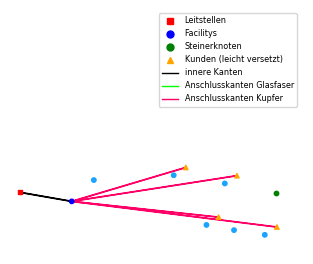
\includegraphics[width=\textwidth]{./Bilder/P2PGK_Naunyn_demand1_duration0}
	\end{minipage}
	\begin{minipage}[b]{0.4\textwidth}
		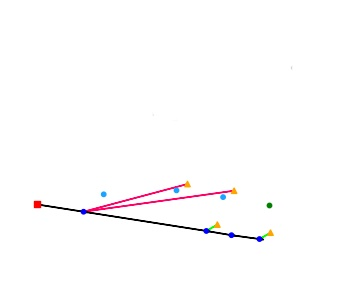
\includegraphics[width=\textwidth]{./Bilder/P2PGK_Naunyn_demand1_5_duration0}
	\end{minipage}
	\begin{minipage}[b]{0.4\textwidth}
		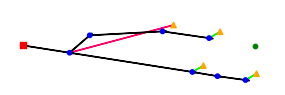
\includegraphics[width=\textwidth]{./Bilder/P2PGK_Naunyn_demand3_5_duration0}
	\end{minipage}
	\begin{minipage}[b]{0.4\textwidth}
		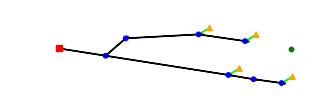
\includegraphics[width=\textwidth]{./Bilder/P2PGK_Naunyn_demand6_5_duration0}
	\end{minipage}
	\caption{Lösung des P2PGK mit verschiedenen Bedarfsfaktoren $d$ auf der Instanz Naunyn. Links oben: $d=1$, rechts oben: $d=1,5$, links unten $d=3,5$, rechts unten: $d=6,5$}
	\label{P2PGK_Naunyn_Bedarf}
\end{figure}

Die gleiche Analyse für Berlin und Vehlefanz fassen wir nun in den Tabellen \eqref{P2PGK_Berlin_Bedarf} und \eqref{P2PGK_Vehlefanz_Bedarf} zusammen.
Dabei steht $A_G$ für die Anzahl der Kunden, die mit Glasfaser angeschlossen werden.
In Berlin gibt es insgesamt 39 Kunden und in Vehlefanz 238 Kunden.

\begin{table}[h]
	\centering
	\begin{minipage}{.35\textwidth}
			\centering
	\begin{tabular}{c|c|c}
		\centering
		d& Kosten & $A_G$ \\	
		\hline
		1& 524.392 & 3 \\
		1,5 & 709.412 & 10 \\
		2 & 834.472 & 15 \\
		2,5 & 1.046.842 & 22 \\
		3 & 1.142.322 & 28 \\
		3,5 & 1.152.122 & 28 \\
		4 & 1.174.552 & 30 \\
		4,5 & 1.220.122 & 33 \\	
		5 & 1.220.122 & 33 \\
		$\infty$ &  1.388.562 & 39 \\
	\end{tabular}
	\label{P2PGK_Berlin_Bedarf}
	\caption{Lösung des P2PGK auf der Instanz Berlin mit veschiedenen Bedarfsfaktoren}
	\end{minipage}
	\hspace{0.5cm}
	\begin{minipage}{0.35\textwidth}
			\centering
		\begin{tabular}{c|c|c}
			\centering
			$d$ & Kosten & $A_G$ \\	
			\hline
			$1$   &   647.608 & 0  \\
			$1,5$ &   647.608 & 0  \\
			$2$   &   826.768 & 3  \\
			$2,5$ &   907.508 & 7  \\
			$3$   & 1.274.782 & 15 \\
			$3,5$ & 1.924.742 & 40 \\
			$4$   & 2.137.362 & 47 \\
			$4,5$ & 2.325.942 & 56 \\
			$5$   & 2.350.572 & 57 \\
			$\infty$ & 7.791.258 & 238 \\ 
		\end{tabular}
		\label{P2PGK_Vehlefanz_Bedarf}
	\caption{Lösung des P2PGK auf der Instanz Vehlefanz mit veschiedenen Bedarfsfaktoren $d$}
	\end{minipage}
\end{table}
\vspace{0.5cm}
In der Tabelle \ref{P2PGK_Berlin_Bedarf} erkennen wir, dass  bei einem Bedarfsfaktor $d$ von nur $1,5$ schon 10 Kunden mit Glasfaser angeschlossen werden und die Anzahl stetig steigt.
Bei einem Wert $d=5$ werden schon 33 von 39 Kunden mit Glasfaser angeschlossen.
Bei der Instanz Vehlefanz hingegen werden bei $d=5$ erst 57 von 238 Kunden mit Glasfaser angeschlossen.
Ingesamt steigt die Anzahl der mit Glasfaser angeschlossenen Kunden deutlich langsamer als bei der Instanz Berlin.

Nun erweitern wir das P2PGK Problem, indem wir zusätzlich noch den Profit für den Anschluss eines Kunden betrachten.
Der monatliche Profit für den Anschluss eines Kunden $k \in K$ beträgt für Glasfaser $p_1(k)$ und für Kupfer $p_2(k)$, im folgenden betrachten wir dies als Profitfunktion $p:K \times \{1,2\} \rightarrow \Q_{ \geq 0 },(k,i) \mapsto p_i(k)$.
Dazu führen wir eine Variable $t$ für die Anzahl der betrachteten Monate ein.
Für $t=0$ entspricht das Problem dem P2PGK wie im Abschnitt zuvor.

Um diese Erweiterung unseres P2PGK Problems zu lösen, übergeben wir dem Algorithmus \ref{alg1} hierbei noch zusätzlich $t$ und $p$ und passen die Kostenfunktion \(c'\) \eqref{first_c_prime} wie folgt an.
\begin{align*}
c': A'' \rightarrow \Q, ij \mapsto \left\{\begin{array}{cl} 
c_{\text{dij}}(lj), & \text{falls } ij = lj \in D \text{ und } j \in F_1\\ 
c_{\text{dij}}(lj)+c(j), & \text{falls } ij = lj \in D \text{ und } j \in F_2\\ 
c(ij) + c(i) - t \cdot p(j,1), & \text{falls } ij \in A_1\\ 
c(ij) - t \cdot p(j,2), & \text{falls } ij \in A_2\\ 
\end{array}
\right.
\end{align*}
Außerdem erweitern wir das Steinerbaum Modell um die Bedingung 
\begin{align*}
	x_{ij} \leq \displaystyle\sum_{j \in K} y_{ij}^t \quad \forall ij \in A \text{ mit } c'(ij) \leq 0.
\end{align*}
Diese Nebenbedingung ist notwendig, da sonst alle Kanten $ij$ mit negativen Kosten ausgewählt werden.
Die Nebenbedingung verhindert dies, da nun nur die Kanten ausgew\"ahlt werden können, welche auch wirklich in dem Fluss vorkommen.
Es ist leicht zu sehen, dass der Algorithmus \ref{alg1} jetzt auch hierfür die optimale Lösung ausgibt. 

\textbf{Auswertung:}
Zuerst stellen wir fest, dass der Profit einen Kunden $k \in K$ mit Glasfaser anzuschließen oft sich nur um 1/3 höher als der Profit p $p_2(k)$. 
Wir betrachten die Veränderung der Ergebnisse in 10-Jahres Schritten, da ein großer Planungshorizont bei diesem Projekt mehr Sinn macht.
Betrachten wir hier nun die Instanz Berlin. Für $t=0$ haben wir Kosten von 524.392 und es werden 3 Kunden mit Glasfaser angeschlossen. Nach 10 Jahren sind die Kosten gesunken auf 366.112 bei gleich bleibender Anzahl von Kunden mit Glasfaseranschluss. Es ist sehr wahrscheinlich, dass sich das Netzwerk hier nicht ändert. Erst bei einem Planungshorizont von 40 Jahren ändert sich das Netzwerk, aber es wird nur ein Kunde mehr mit Glasfaser angeschlossen. Da sich in 40 Jahren sehr viel ändern kann, ist es nicht sinnvoll den Profit mit in die Planung einzubeziehen. Für Naunyn und Vehlefanz ergibt die Analyse des Profit dasselbe. Also sollte das Netzwerk aufgebaut werden, dass auch herauskommt, wenn man ohne Profit rechnet. Die genauen 

Zusammenfassend ist es in unseren Instanzen beim P2P- Problem wichtiger eine steigende Nachfrage zu betrachten als den Profit für

\section{Point-to-multipoint communication}
In diesem Kapitel behandeln wir die Point-to-multipoint Problemstellung.  Dabei betrachten wir erst den Fall, dass jeder Kunde durch eine Glasfaserkante angeschlossen wird. In dem darauffolgenden Abschnitt k\"onnen Kunden sowohl mit Glasfaser- als auch mit Kupferkabeln an das Netzwerk angeschlossen werden. Im letzten Abschnitt erweitern wir das P2MP mit Glasfaser und Kupfer Problem, indem wir auch monatliche Profit f\"ur den Anschluss eines Kunden mit einberechnen und indem wir unterschiedliche Nachfrage an Bandbreite in unser Modell einbeziehen.

 
 \subsection{Point-to-multipoint mit Glasfaser}
 
 
 Die Problemstellung beim P2MP mit Glasfaser (P2MPG) ist es,  jeden Kunden \"uber einen Glasfaseranschluss in das Netzwerk einzubinden und dabei die entstehenden Kosten zu minimieren. Anders als beim P2PG braucht nicht jeder Kunde eine eigene Leitung (bis auf die lezte Meile), sondern es k\"onnen auch Kabel durch einen Splitter in mehrer Kabel aufgeteilt werden.  Das heisst, bei diesem Problem  m\"ussen wir wieder zuerst eine Leitstelle aus $L$ ausw\"ahlen und dann jeden Kunden an eine Facility anbinden, welche durch eine Glasfaserleitung  an diese Leitstelle angebunden ist. Falls nun ein Splitter in einem Knoten installiert wird und ein Glasfaserkabel in diesen Knoten geht, dann k\"onnen bis zu $a$-viele Kanten aus diesem Knoten herausgehen, wobei $a$ entweder 4 oder 16 ist.

Das Problem lösen wir, indem wir das folgende Model für jede Leistelle $l \in L $ mit Gurobi lösen
 und dann die kostenminimale L\"oesung davon ausw\"ahlen. Sei dazu $A:= I\backslash I_L \cup A_1$, wobei $I_L$ die Menge der ausgehenden Kanten aus den nicht ausgewählten Leitstellen ist.
Die Entscheidungsvariable $y_{ij}^t \in \{0,1\}\; \forall ij \in A, t \in K$ modelliert einen Fluss von der Leitstelle $l$ zu dem Kunden $t$ für jeden Kunden. Falls $y_{ij}^t=1$ ist, heißt das, dass der Fluss von $l$ nach $t$ über die Kante $ij$ fließt.
Die Variable $x_{ij} \in \Z_{\geq 0} \; \forall ij \in A $ gibt an, wie häufig die Kante in dem Netzwerk auftritt, bzw. wie häufig wir eine Kante kaufen müssen. Außerdem haben wir die binäre Entscheidungsvariable $s_i \in \{0,1\}$ für $i \in F \cup S$ eingeführt. Diese gibt an, ob in dem Knoten $i$ ein Splitter installiert wird ($s_i=1$) oder nicht ($s_i=0$). In dem Model wollen wir nun die Kosten für die Installation eines Splitter und die Kosten für die Kanten minimieren. Daf\"ur haben wir die Kostenfunktion \eqref{Kostenfunktion} ver\"andert und haben die Kosten für den Glasfaseranschluss auf die Kantenkosten der Anschlusskanten für Glasfaser addiert.
\begin{align}
\label{KostenfunktionP2MP}
c': A \rightarrow \Q, ij  \mapsto \left\{\begin{array}{cl} 
c(ij), & \text{falls } ij \in I\backslash I_L\\ 
c(ij)+c(j), & \text{falls } ij \in A_1\\ 
\end{array}
\right.
\end{align}
Also ergibt sich die folgende Minimierungsfunktion und insgesamt das folgende Modell.


 \bigskip
 $\min \displaystyle\sum_{ij \in A} c'(ij) x_{ij} + \displaystyle\sum_{i \in F \cup S} c_s s_i $
 \begin{align*}
 \begin{array}{rcrcrcll}
 \textrm{s.t.}  
&& &\displaystyle\sum_{ji \in A} y_{ji}^t - \displaystyle\sum_{ij \in A} y_{ij}^t& = & \left\{\begin{array}{cl} 
 -1, & \text{falls } i=l\\ 
 1, & \text{falls } i=t\\ 
 0, & \text{sonst.}\\ 
 \end{array}
 \right. & \forall t \in K & (1) \\
 &&& y_{ij}^t & \leq & x_{ij} & \forall ij \in A, t\in K & (2)\\
 &&& s_i &\leq& \displaystyle\sum_{ji \in A} x_{ji}& \forall  i \in S \cup F& (3)\\ 
 &0&\geq&\displaystyle\sum_{ji \in A} x_{ji} - \displaystyle\sum_{ij \in A} x_{ij}&\geq& -(a-1)s_i & \forall i \in S \cup F& (4)\\
 &&& y_{ij}^t & \in & \{0,1 \}& \forall ij \in A, t \in K & (5)\\
 &&& x_{ij} & \in & \Z _{\geq 0}& \forall ij \in A, t \in K & (6)\\
 &&& s_i & \in & \{ 0,1 \} & \forall i \in F \cup S & (7) \\
 \end{array}
 \end{align*}
 Die Nebenbedienung (1) modelliert, wie im Steinerbaum Problem mit Flussbedingung, einen Fluss für jeden Kunden $t \in K$ von der Leitstelle $l$ zu dem Kunden. Dabei gibt die Formel $\displaystyle\sum_{ji \in A} y_{ji}^t - \displaystyle\sum_{ij \in A} y_{ij}^t$ die Flusserhaltung an. Falls diese Formel gleich -1 eins ist, geht als ein Fluss aus dem Knoten heraus. Dabei geht keine Kante in die Leitstelle ein, da die Leitstelle nur ausgehende Kanten besitzt. Das gleiche gilt für die Kunden, diese haben nur eingehende Kanten und somit gilt, falls die Formel gleich 1 ist, dass genau ein Flusskante in den Kundenknoten geht. Die zweite Nebenbedingung stellt sicher, dass falls wir eine Kante in dem Fluss von $l$ nach $t$ benutzen, wird diese Kante auch in unserem Netzwerk gekauft. Falls wir einen Splitter auf einem Knoten $i \in S \cup F$ benutzen, braucht dieser Splitter auch ein Kabel, dass er splitten kann. Dies gewährleistet Bedingung (3). Außerdem besitzen die $x_{ij}$-Variablen auch Flusserhaltung, modelliert in Bedingung (4). Dies ist notwendig, da wir nur dann die Kabel aufteilen können, wenn wir auch einen Splitter installieren. Falls wir keinen Splitter installieren, also $s_i=0$, müssen genauso viele Kabel in den Knoten rein gehen, wie auch wieder raus gehen, dh. $\displaystyle\sum_{ji \in A} x_{ji} - \displaystyle\sum_{ij \in A} x_{ij}=0$. Falls wir einen Splitter installieren ($s_i=1$), können bis zu $a$ Kanten aus diesem Knoten heraus gehen. Deshalb muss die Flusserhaltung der $x_{ij}$ größer als $-(a-1)$ sein. \TODO NEBENBEDINUNG(4)KACKE
 Die Nebenbedienungen (5)-(7) wurden über dem Modell erklärt.
  
  Falls wir $a=1$ w\"ahlen l\'ost dieses  Modell das P2PG Problem.
  
 \TODO wieso ist das die optimale lösung also wieso schränken wir keine vll besseren 
 lösungen ein
 
  Falls wir $a=1$ w\"ahlen l\'ost dieses  Modell das P2PG Problem.
 
 \TODO Ergebnisse beschreiben +splitter 4 oder 16 oder noch andere splitter
 \begin{table}[h]
 	\centering
 	\begin{tabular}{c|c|c}
 		Instanz & Naunyn & Berlin \\	
 		\hline
 		 Kosten für $a=4$ & 449.255,33 & 705.182,94 \\
 		 Laufzeit auf PC1 & 0,046s & 2h 14m \\
 		 \hline
 		Kosten für $a=16$ & \TODO & \\
 		Laufzeit auf PC2 &  & \\
 	\end{tabular}
 	\label{P2MPG}
 	\caption{Ergebnisse des P2MPG f\"ur Naunyn und Berlin} 
 \end{table}
 
 \begin{table}[h]
 	\centering
 	\begin{tabular}{c|c|c|c|c}
 		Vehlefanz & untere Schranke & obere Schranke & Gap & Laufzeit auf PC1\\	
 		\hline
 		 Kosten für $a=4$ & 1.528.315,57 & 1.537.043,86 & 0,568\% & 10h 8m\\
 		 \hline
 		Kosten für $a=16$ & \TODO &  & &  \\
 	\end{tabular}
 	\label{P2MPG}
 	\caption{Ergebnisse des P2MPG f\"ur Vehlefanz} 
 \end{table}
 \TODO vergleich von 1, 4 und 16 
 
 \subsection{Point-to-multipoint mit Glasfaser und Kupfer}
\TODO PROBLEM beschreibung+einleitung

Diese Problem lösen wir mit einer Erweiterung des linearen Programms des P2MPG Problems. Sei der Graph \TODO FALSCHER GRAPH!!! und die Kosten \eqref{KostenfunktionP2MP} also gegeben wir vorher und  seinen die Entscheidungsvariablen $y_{ij}^t,x_{ij}$ und $s_i$ definiert wie in dem P2MPG Model. Wir fügen noch eine Entscheidungsvariable $m_i \in \{0,1\} \forall i \in F_2$. In jeder Facility von Typ 2 kann bei diesem Problem noch ein DSL-Zugangsmultiplexer installiert werden. Genau dann wenn $m_i=1$ ist, wird ein Multiplexer installiert. Die Zielfunktion des Models wird deswegen noch durch den Summand $\displaystyle\sum_{i \in F_2} c(i) m_i$ erweitert. Insgesamt ergibt sich folgendes Model:

  \bigskip
  $\min \displaystyle\sum_{ij \in A} c'(ij) x_{ij} + \displaystyle\sum_{i \in F \cup S} c_s s_i + \displaystyle\sum_{i \in F_2} c(i) m_i$
  \begin{align*}
  \begin{array}{rcrcrcll}
  \textrm{s.t.}  
  && &\displaystyle\sum_{ji \in A} y_{ji}^t - \displaystyle\sum_{ij \in A} y_{ij}^t& = & \left\{\begin{array}{cl} 
  -1, & \text{falls } i=r\\ 
  1, & \text{falls } i=t\\ 
  0, & \text{sonst.}\\ 
  \end{array}
  \right. & \forall t \in K & (1) \\
  &&& y_{ij}^t & \leq & x_{ij} & \forall ij \in A, t\in K & (2)\\
    &&& s_i &\leq& \displaystyle\sum_{ji \in A} x_{ji}& \forall  i \in F \cup S & (3)\\ 
  &0&\geq&\displaystyle\sum_{ji \in A} x_{ji} - \displaystyle\sum_{ij \in A} x_{ij}&\geq& -(a-1)s_i & \forall i \in S \cup F_1& (4)\\
   &0&\geq&\displaystyle\sum_{ji \in A} x_{ji} -m_i - \displaystyle\sum_{ij \in I \cup A_1} x_{ij}&\geq& -(a-1)s_i & \forall i \in F_2& (4')\\
   &&&s_i+m_i & \leq & 1 & \forall i \in F_2 & (8)\\
   &&&x_{ij}& \leq & m_i & \forall i \in F_2 & (9) \\
    &&& y_{ij}^t & \in & \{0,1 \}& \forall ij \in A, t \in K & (5)\\
    &&& x_{ij} & \in & \Z_{\geq 0} & \forall ij \in A, t \in K & (6)\\
    &&& s_i & \in & \{ 0,1 \} & \forall i \in F \cup S & (7) \\
    &&& m_i & \in & \{ 0,1 \} & \forall i \in F_2 & (10) \\
  \end{array}
  \end{align*}
  
  Die Nebenbedingungen (4) aus dem P2MPG Model bleibt für die Knoten $S \cup F$ die Gleiche. In den Knoten aus $F_2$ können wir nun auch eine Multiplexer installieren. Dies müssen wir auch bei der Flusserhaltung der $x_{ij}$ beachten. Die Nebenbedienungen (4') modelliert den Fluss der $x_{ij}$ für die Knoten $i \in F_2$. Falls ein Splitter installiert wird, kann kein Multiplexer installiert werden und die Bedienungen ist wie im P2MPG Model. Falls ein Multiplexer $i \in F_2$ ($m_i=1$) installiert wird, geht ein Glasfaserkabel in den Multiplexer und es k\'onnen unendlich viele Kupferkabel, also Anschlusskanten von Typ 2, hinaus gehen. Jedoch muss die Flusserhaltung f\'ur die inneren Kanten und die Anschlusskanten von Typ 1 erhalten bleiben. Dies modelliert die Gleichung $\displaystyle\sum_{ji \in A} x_{ji} -1 - \displaystyle\sum_{ij \in I \cup A_1} x_{ij}=0$.  In jedem Knoten aus $F_2$ kann entweder ein Multiplexer oder ein Splitter installiert werden, nicht beides gleichzeitig. Dies wird durch Nebenbedingung (8) sichergestelllt. Ausserdem d\'urfen nur Kupferkabel aus einer Facility gehen, falls auch ein Multiplexer installiert ist. Dies wird in Nebenbedingnung (9) modelliert. Die Entscheidungsvariablen (5)-(7) und (10)
wurden schon oben dr\"uber erkl\'art.   
   \TODO+wieso ist das die optimale lösung also wieso schränken wir keine vll besseren lösungen ein
   \TODO Ergebnisse beschreiben
 \begin{table}[h]
	\centering
	\begin{tabular}{c|c|c|c}
		Instanz & Naunyn & Berlin & Vehlefanz \\	
		\hline
		Kosten für $a=4$ & 397.662,0 & 474.909,28 & 587.503,28 \\
		Laufzeit auf PC1 & 0,03s & 7m 13s & 14m 55s \\
		\hline
		Kosten für $a=16$ & \TODO &  &  \\
		Laufzeit auf PC2 &  &  & \\
	\end{tabular}
	\label{P2MPGK}
	\caption{Ergebnisse des P2MPGK} 
\end{table}
\TODO vergleich von 1,4 und 16 
   
 \subsection{Erweiterung des P2MPGK}
 Wie beim P2PGK-Problem in Abschnitt \ref{Erweiterung des P2PGK} kann man auch hier mit Profiten f\"ur jeden Kunden rechnen oder einen steigenden Bedarf an Bandbreite betrachten.
 
 Um den voraussichtlich steigenden Bedarf an Bandbreite eines Kunden zu modellieren, haben wir genau wie in Abschnitt \ref{Erweiterung des P2PGK} den angegebenen Bedarf mit verschiedenen Werten $d$ multipliziert und dann die Kanten gel\"oscht, die diesen Bedarf der Kunden nicht decken (siehe Abschnitt \ref{preprocess}), um dann mit diesem neuen Graphen das P2PGK-Problem zu l\"osen.
 
 \textbf{Auswertung:} \TODO
 
  
Nun erweitern wir das P2PGK Problem, indem wir zusätzlich noch den Profit für den Anschluss eines Kunden  betrachten.
 Auch hier gehen wir genauso vor wie Abschnitt \ref{Erweiterung des P2PGK}.  Wieder gibt die Varibale  $t$  den Planungshorizont in Monaten an. Wir \"ubergeben unserem Model also noch die Variable $t$ und die Profitfunktion $p$. Ausserdem \"andern wir die Kostenfunktion \eqref{KostenfunktionP2MP}  zu folgender Funktion:
 \begin{align*}
  c'': A  \rightarrow \Q,  ij  \mapsto \left\{\begin{array}{cl} 
 c'(ij), & \text{falls } ij \in I\backslash I_L \\ 
  c'(ij) -t  \cdot p_1(j), & \text{falls } ij \in I\backslash A_1 \\ 
    c'(ij) -t \cdot p_2(j), & \text{falls } ij \in I\backslash A_2 \\ 
\end{array}  \right.
 \end{align*}
 Ausserdem erweitern wir das P2MPGK Model durch die Nebenbedingung 
 \begin{align*}
 x_{ij} \leq \displaystyle\sum_{t \in K} y_{ij}^t \quad \forall ij \in A \text{ mit } c''(ij) \leq 0
 \end{align*}
 
 \textbf{Auswertung:} \TODO
 
 \TODO erweiterung verschiedene Splitter mit verschiedenen Kosten
 
 \section{Zusammenfassung/Fazit}
 \TODO Graphische verschauen der verschiedenen Ergebnisse der verschiedenen Probleme
 
 \begin{figure}[!htbp]
 	\begin{tikzpicture}
 	\begin{axis}[
 	symbolic x coords={P2PGK1,P2PGK1.5,P2PGK3,P2PG,P2MPG,P2MPGK1, P2MPGK1.5,P2MPGK3},
 	x tick label style={rotate=45,anchor=east},
 	height=8cm, width=15cm,
 	bar width=0.4cm,
 	enlarge x limits=true,
 	ylabel=Kosten]
 	\addplot[ybar,fill=red] coordinates {
 		(P2PGK1,      524392)
 		(P2PGK1.5,   709412)
 		(P2PGK3,        1142322)
 		(P2PG,        1388562)};
 	\addplot[ybar,fill=blue] coordinates {
 		(P2MPG,   705182)
 		(P2MPGK1,      474909)
 		(P2MPGK1.5,   5466)
 		(P2MPGK3,    345646)};
 	\end{axis}
 	\end{tikzpicture}
 	\caption{\"Ubersicht der Ergebnisse der Instanz Berlin}
 \end{figure}
 
  \begin{figure}[!htbp]
 	\begin{tikzpicture}
 	\begin{axis}[
 	symbolic x coords={P2PGK1,P2PGK1.5,P2PGK3,P2PG,P2MPG,P2MPGK1, P2MPGK1.5,P2MPGK3},
 	x tick label style={rotate=45,anchor=east},
 	height=8cm, width=15cm,
 	bar width=0.4cm,
 	enlarge x limits=true,
 	ylabel=Kosten]
 	\addplot[ybar,fill=red] coordinates {
 		(P2PGK1,      524392)
 		(P2PGK1.5,   709412)
 		(P2PGK3,        1142322)
 		(P2PG,        1388562)};
 	\addplot[ybar,fill=blue] coordinates {
 		(P2MPG,   705182)
 		(P2MPGK1,      474909)
 		(P2MPGK1.5,   1388562)
 		(P2MPGK3,   138856)};
 	\end{axis}
 	\end{tikzpicture}
 	\caption{\"Ubersicht der Ergebnisse der Instanz Naunyn}
 \end{figure}
 
  \begin{figure}[!htbp]
 	\begin{tikzpicture}
 	\begin{axis}[
 	symbolic x coords={P2PGK1,P2MPGK1,P2MPGK1.5,P2MPGK3,P2PGK1.5,P2PGK3,P2MPG,P2PG},
 	x tick label style={rotate=45,anchor=east},
 	height=8cm, width=15cm,
 	bar width=0.4cm,
 	enlarge x limits=true,
 	ylabel=Kosten]
 	\addplot[ybar,fill=red] coordinates {
 		(P2PGK1,      397622)
 		(P2PGK1.5,   442842)
 		(P2PGK3,        442842)
 		(P2PG,        480722)};
 	\addplot[ybar,fill=blue] coordinates {
 		(P2MPG,   449255)
 		(P2MPGK1,      397622)
 		(P2MPGK1.5,   427533)
 		(P2MPGK3,   427533)};
 	\end{axis}
 	\end{tikzpicture}
 	\caption{\"Ubersicht der Ergebnisse der Instanz Naunyn}
 \end{figure}
 
\newpage
\bibliographystyle{babplain-lf}
\renewcommand{\refname}{Literaturverzeichnis}
\bibliography{literatureProject1}
\thispagestyle{empty}
\newpage
\appendix
\section*{Abbildungsverzeichnis}
\textbf{P2PG:}
\begin{figure}[!htbp]
	\label{p2pg_n_pic}
	\begin{center}
		\begin{minipage}{10.0cm}
			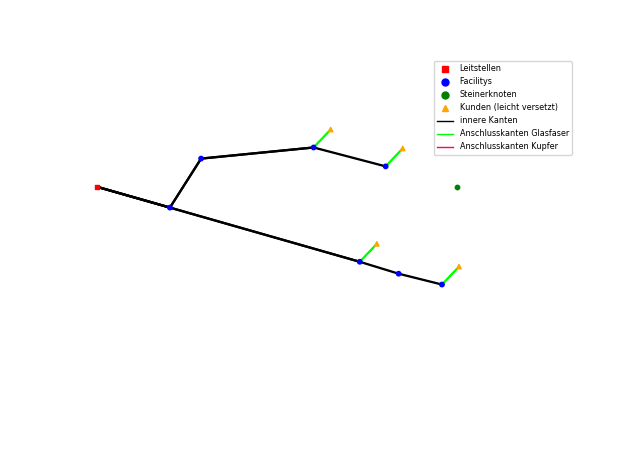
\includegraphics[width=1\textwidth]{./Bilder/P2PG_Naunyn}
			\caption{Lösung des P2PG Problems auf der Instanz Naunyn}
		\end{minipage}
	\end{center}
\end{figure}

\begin{figure}[!htbp]\label{p2pg_b_pic}
\begin{center}
	\begin{minipage}{15.0cm}
		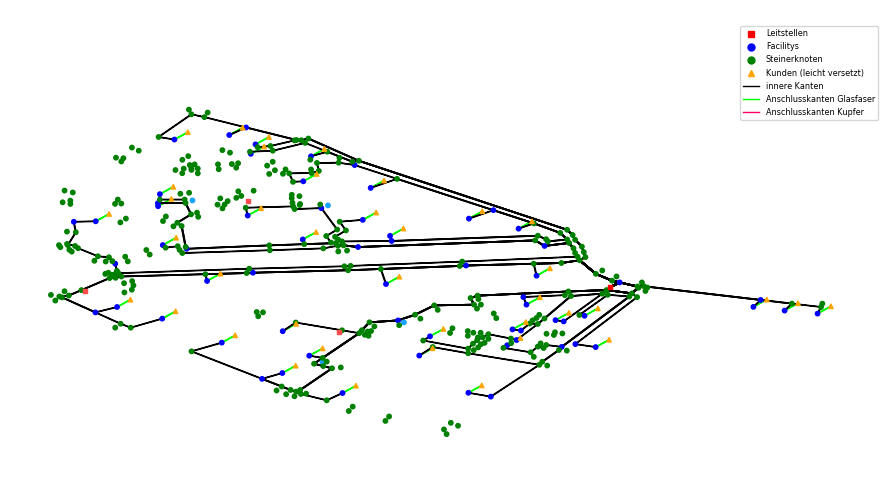
\includegraphics[width=1\textwidth]{./Bilder/P2PG_Berlin}
		\caption{Lösung des P2PG Problems auf der Instanz Berlin}
	\end{minipage}
\end{center}
\end{figure}

\begin{figure}[!htbp]\label{p2pg_v_pic}
\begin{center}
	\begin{minipage}{15.0cm}
		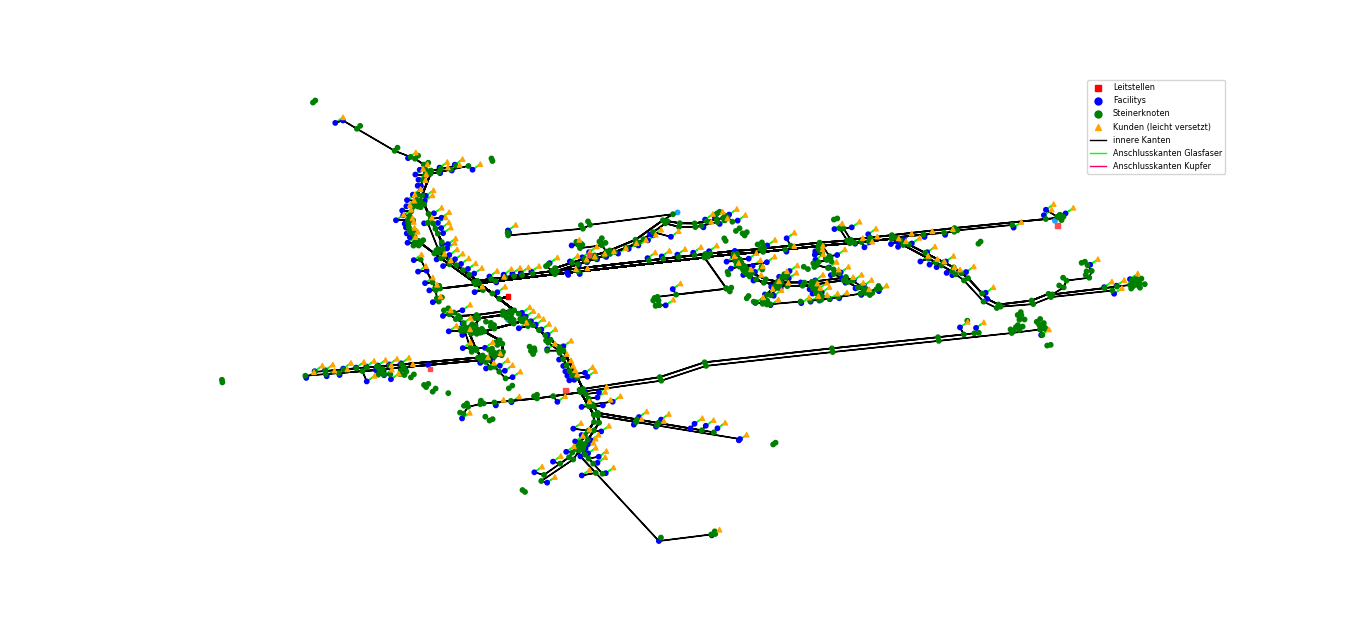
\includegraphics[width=1\textwidth]{./Bilder/P2PG_Vehlefanz}
		\caption{Lösung des P2PG Problems auf der Instanz Vehlefanz}
	\end{minipage}
\end{center}
\end{figure}

\textbf{P2PGK:}

\begin{figure}[!htbp]\label{p2pgk_n_pic}
	\begin{center}
		\begin{minipage}{10.0cm}
			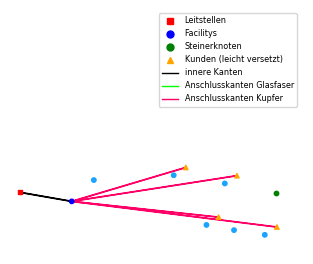
\includegraphics[width=1\textwidth]{./Bilder/P2PGK_Naunyn_demand1_duration0}
			\caption{Lösung des P2PGK Problems auf der Instanz Naunyn}
		\end{minipage}
	\end{center}
\end{figure}

\begin{figure}[!htbp]\label{p2pgk_b_pic}
	\begin{center}
		\begin{minipage}{15.0cm}
			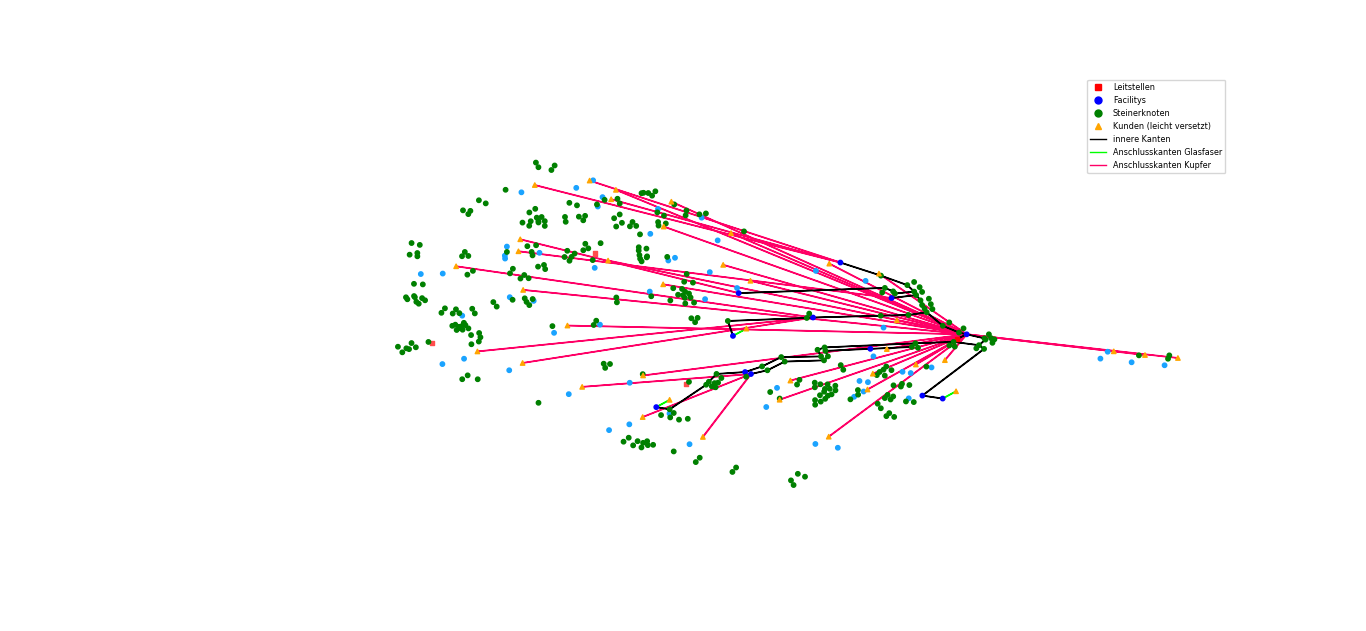
\includegraphics[width=1\textwidth]{./Bilder/P2PGK_Berlin_demand1_duration0}
			\caption{Lösung des P2PGK Problems auf der Instanz Berlin}
		\end{minipage}
	\end{center}
\end{figure}

\begin{figure}[!htbp]\label{p2pgk_v_pic}
	\begin{center}
		\begin{minipage}{15.0cm}
			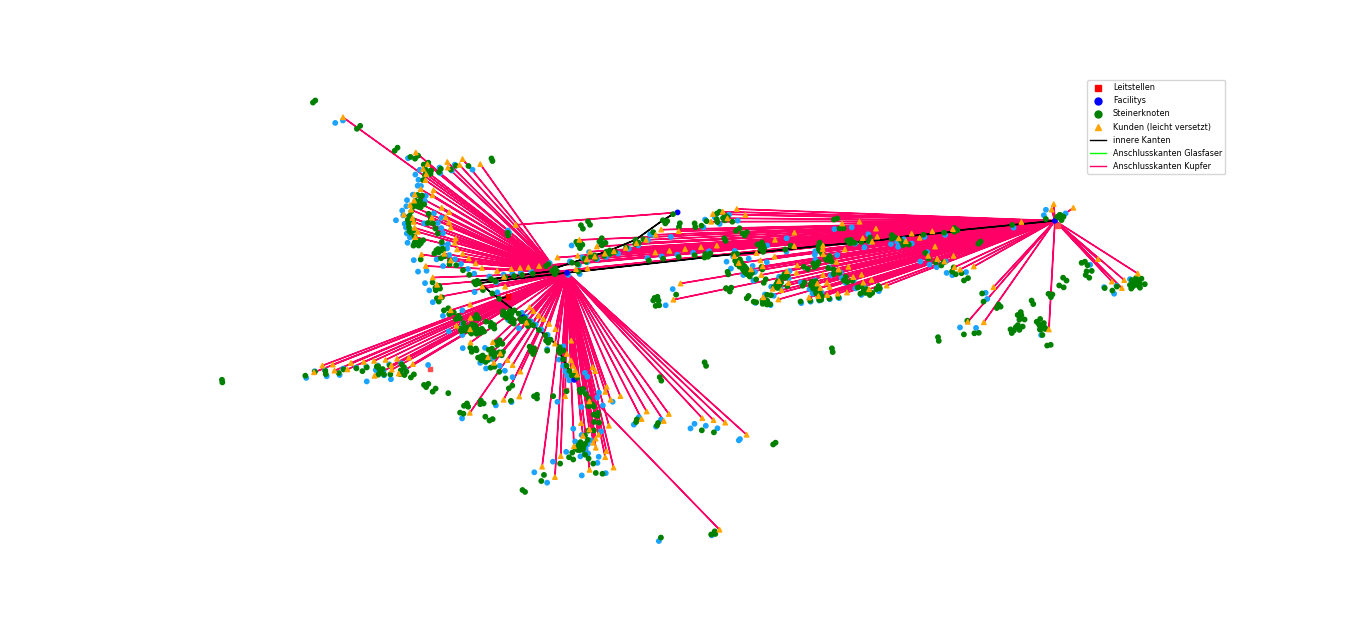
\includegraphics[width=1\textwidth]{./Bilder/P2PGK_Vehlefanz_demand1_duration0}
			\caption{Lösung des P2PGK Problems auf der Instanz Vehlefanz}
		\end{minipage}
	\end{center}
\end{figure}

\addcontentsline{toc}{section}{Abbildungsverzeichnis}
\newpage
\section*{Anhang}
\subsection*{Steinerbaum Model mit Fluss Formulierung}
\textbf{Gegeben:} Graph $G=(V,A)$, Menge an Terminalen $T \subseteq V $, Wurzel $r \in T$, Kostenfunktion $c:A \rightarrow \Q$\\
\textbf{Gesucht:} Teilgraph von $G$ (Steinerbaum), der alle Knoten aus $T$ verbindet und bei dem die Summe der Kosten minimal ist\\
\textbf{Entscheidungsvariablen:}\\
\begin{tabular}{lll}
	$y_{ij}^t \in \{0,1\}$ &$\forall ij \in A, t\in T $ & modelliert einen Fluss für jeden Terminal $t$ von der Leitstelle $l$\\
	&& zum Terminal $t$\\
	$x_{ij} \in \{0,1\}$ & $\forall ij \in A$ &gibt an, ob die Kante $ij$ Teil des Steinerbaums ist ($x_{ij}=1$)\\
	&& oder nicht ($x_{ij}=0$)\\
\end{tabular}\\
\textbf{Model:}
$\min \displaystyle\sum_{ij \in A} c_{ij} x_{ij} $
\begin{align}
\begin{array}{rcrcrcll}
\textrm{s.t.}  
&& &\displaystyle\sum_{ji \in A} y_{ji}^t - \displaystyle\sum_{ij \in A} y_{ij}^t& = & \left\{\begin{array}{rl} 
-1, & \text{falls } i=l\\ 
1, & \text{falls } i=t\\ 
0, & \text{sonst}\\ 
\end{array}
\right. & \forall t \in T & (1) \\
  &&& y_{ij}^t & \leq & x_{ij} & \forall ij \in A, t\in T & (2)\\
&&& y_{ij}^t & \in & \{0,1 \}& \forall ij \in A , t \in T& (3)\\
&&& x_{ij} & \in & \{0,1\}& \forall ij \in A & (4)\\
\end{array}
\label{SteinerbaumModel}
\end{align}


\subsection*{P2PGK mit Profit}
Hier sind die Ergebnisse des P2PGK-Problems mit Profit. Dabei ist $A_G$ die Anzahl der Kunden mit einem Glasfaseranschluss.
\begin{table}[!htbp]
	\centering
	\begin{tabular}{c|c|c}
		\centering
		Jahre & Kosten & $A_G$ \\	
		\hline
		$0$   	 &  524.392 & 3  \\
		$10$ 	&   366.112& 3  \\
		$20$   	&   207.832 & 3  \\
		$30$    &   49.552 & 3  \\
		$40$    & $-111.448$ & 4 \\
	\end{tabular}
	\label{P2PGKProfit}
	\caption{Ergebnisse des P2PGK mit Profit f\"ur Berlin} 
\end{table}

\begin{table}[!htbp]
	\centering
	\begin{tabular}{c|c|c}
		\centering
		Jahre & Kosten & $A_G$ \\	
		\hline
		$0$   	 &  397.662& 0  \\
		$10$ 	&  382.062 & 0  \\
		$20$   	&  366.462  & 0  \\
		$30$    &  350.862 & 0  \\
		$40$    &  335.262  & 0 \\
	\end{tabular}
	\label{P2PGKProfitN}
	\caption{Ergebnisse des P2PGK mit Profit f\"ur Naunyn} 
\end{table}

\begin{table}[!htbp]
	\centering
	\begin{tabular}{c|c|c}
		\centering
		Jahre & Kosten & $A_G$ \\	
		\hline
		$0$   	 & 647608  &0  \\
		$10$ 	&  426.328 & 0  \\
		$20$   	&  205.048  & 0  \\
		$30$    & $-16.232$& 0  \\
		$40$    &  $-237.512$ & 0 \\
	\end{tabular}
	\label{P2PGKProfitV}
	\caption{Ergebnisse des P2PGK mit Profit f\"ur Vehlefanz} 
\end{table}
\vspace{3cm}
\subsection*{P2MPGK mit Bedarfsfaktor}
Hier sind die Ergebnisse des P2PGK-Problems mit Bedarfsfaktor $d$. Dabei ist $A_G$ die Anzahl der Kunden mit einem Glasfaseranschluss.
\begin{table}[!htbp]
	\centering
		\begin{tabular}{c|c|c}
	\centering
	$d$ & Kosten & $A_G$ \\	
	\hline
	$1$   	 &  397.622 & 0  \\
	$1,5$ 	&   $427.553,11$  & 2  \\
	$2$   	&   $427.553,11$ & 2  \\
	$2,5$   	&   $427.553,11$ & 2  \\
	$3$    &   $427.553,11$ & 2  \\
	$3,5$   	&   $445.743,11$ & 3  \\
	$4$   	&   $445.743,11$& 3  \\
	$4,5$    & $445.743,11$ & 3 \\
	$5$   	&   $445.743,11$& 3  \\
\end{tabular}
	\label{P2MPGKBedarfN}
	\caption{Ergebnisse des P2MPGK mit Bedarfsfaktor $d$ f\"ur Naunyn} 
\end{table}

\begin{table}[!htbp]
			\centering
			\begin{tabular}{c|c|c}
				\centering
				$d$ & Kosten & $A_G$ \\	
		\hline
	$1$   	 &  \TODO& 0  \\
	$1,5$ 	&   $427.553,11$  & 2  \\
	$2$   	&   $427.553,11$ & 2  \\
	$2,5$   	&   $427.553,11$ & 2  \\
	$3$    &   $427.553,11$ & 2  \\
	$3,5$   	&   $445.743,11$ & 3  \\
	$4$   	&   $445.743,11$& 3  \\
	$4,5$    & $445.743,11$ & 3 \\
	$5$   	&   $445.743,11$& 3  \\	
			\end{tabular}
			\label{P2PGKBedarfB}
			\caption{Ergebnisse des P2MPGK mit Bedarfsfaktor $d$ f\"ur Berlin} 
\end{table}

\begin{table}[!htbp]
	\centering
	\begin{tabular}{c|c|c}
		\centering
		$d$ & Kosten & $A_G$ \\	
		\hline
		$1$   	 &  397.622 & 0  \\
		$1,5$ 	&   $427.553,11$  & 2  \\
		$2$   	&   $427.553,11$ & 2  \\
		$2,5$   	&   $427.553,11$ & 2  \\
		$3$    &   $427.553,11$ & 2  \\
		$3,5$   	&   $445.743,11$ & 3  \\
		$4$   	&   $445.743,11$& 3  \\
		$4,5$    & $445.743,11$ & 3 \\
		$5$   	&   $445.743,11$& 3  \\	
	\end{tabular}
	\label{P2PGKBedarfV}
	\caption{Ergebnisse des P2MPGK mit Bedarfsfaktor $d$ f\"ur Vehlefanz} 
\end{table}
\vspace{5cm}
\subsection*{P2MPGK mit Profit}
Hier sind die Ergebnisse des P2MPGK-Problems mit Profit. Dabei ist $A_G$ die Anzahl der Kunden mit einem Glasfaseranschluss.
\begin{table}[!htbp]
	\centering
	\begin{tabular}{c|c|c}
		\centering
		Jahre & Kosten & $A_G$ \\	
		\hline
		$0$   	 &  474.909,28 & 3  \\
		$10$ 	&  316.320,18 & 5  \\
		$20$   	&   145.851,1 & 7  \\
		$30$    &   $ -34.146,17$	& 15  \\
		$40$    & $-235002,54$ &  24 \\
	\end{tabular}
	\label{P2MPGKProfit}
	\caption{Ergebnisse des P2MPGK mit Profit f\"ur Berlin} 
\end{table}

\begin{table}[!htbp]
	\centering
	\begin{tabular}{c|c|c}
		\centering
		Jahre & Kosten & $A_G$ \\	
		\hline
		$0$   	 &  \TODO& 0  \\
		$10$ 	&  382.062 & 0  \\
		$20$   	&  366.462  & 0  \\
		$30$    &  350.862 & 0  \\
		$40$    &  335.262  & 0 \\
	\end{tabular}
	\label{P2MPGKProfitN}
	\caption{Ergebnisse des P2MPGK mit Profit f\"ur Naunyn} 
\end{table}

\begin{table}[!htbp]
	\centering
	\begin{tabular}{c|c|c}
		\centering
		Jahre & Kosten & $A_G$ \\	
		\hline
		$0$   	 & \TODO  &0  \\
		$10$ 	&  426.328 & 0  \\
		$20$   	&  205.048  & 0  \\
		$30$    & $-16.232$& 0  \\
		$40$    &  $-237.512$ & 0 \\
	\end{tabular}
	\label{P2MPGKProfitV}
	\caption{Ergebnisse des P2MPGK mit Profit f\"ur Vehlefanz} 
\end{table}


\addcontentsline{toc}{section}{Anhang}
\thispagestyle{empty}


\end{document}
